% !TEX TS-program = xelatex
% !TEX encoding = UTF-8 Unicode

% Tennessee Technological University
% ME4020 - Fall 2022
% Tristan Hill - August 29, 2022
% Gears Review

\documentclass[fleqn]{beamer} % for presentation (has nav buttons at bottom)

% custom preamble
\usepackage{/home/thill/courses/machine_design/machine_design_lecture}

\newcommand{\MNUM}{1\hspace{2mm}} % Module number
\newcommand{\TNUM}{1\hspace{2mm}} % Topic number 
\newcommand{\moduletitle}{Loads Analysis} 
\newcommand{\lecturetitle}{Gears Review} 

\newcommand{\sectiontitleI}{Overview} % More Titles and Stuff
\newcommand{\sectiontitleII}{Law of Gearing}
\newcommand{\sectiontitleIII}{Gears and Loads}
\newcommand{\sectiontitleIV}{Examples}

\author{ME4020 - Applied Machine Design}
\title{\GD Module \MNUM - \moduletitle}
\date{Mechanical Engineering\vspc Tennessee Technological University}

\begin{document}

\lstset{language=MATLAB,basicstyle=\ttfamily\small,showstringspaces=false}

\frame{\titlepage \center\begin{framed}\Large \textbf{\lecturetitle}\end{framed} \vspace{5mm}}

% Section 0 - Outline
\frame{
	
	\large \textbf{\lecturetitle} \vspace{3mm}\\
	
	\begin{itemize}
	
		\item \hyperlink{sectionI}{\color{black}\sectiontitleI}	\vspace{3mm} % Section I
		\item \hyperlink{sectionII}{\color{black}\sectiontitleII}	\vspace{3mm} % Section II
		\item \hyperlink{sectionIII}{\color{black}\sectiontitleIII}	\vspace{3mm} %Section III
		\item \hyperlink{sectionIV}{\color{black}\sectiontitleIV}	\vspace{3mm} %Section IV
		%\item \hyperlink{sectionV}{\color{black}\sectiontitleV} %Section IV	
	
	\end{itemize}

}

% Section I
\section{\sectiontitleI}

	% Section I - Frame I
	\begin{frame}[label=sectionI] \small
		\frametitle{\sectiontitleI}	
		Primary Purpose:
		\begin{itemize}
			\item 
			\item
			\item
        \end{itemize}

        Applications:
        \begin{itemize}
				\item 
				\item
				\item
        \end{itemize}

	\end{frame}

	% Section I - Frame II
	\begin{frame}[label=sectionI] \small
		\frametitle{\sectiontitleI}	
		
		\begin{tabular}{|c|c|c|} 

			Example& Type& Application \\ \hline
			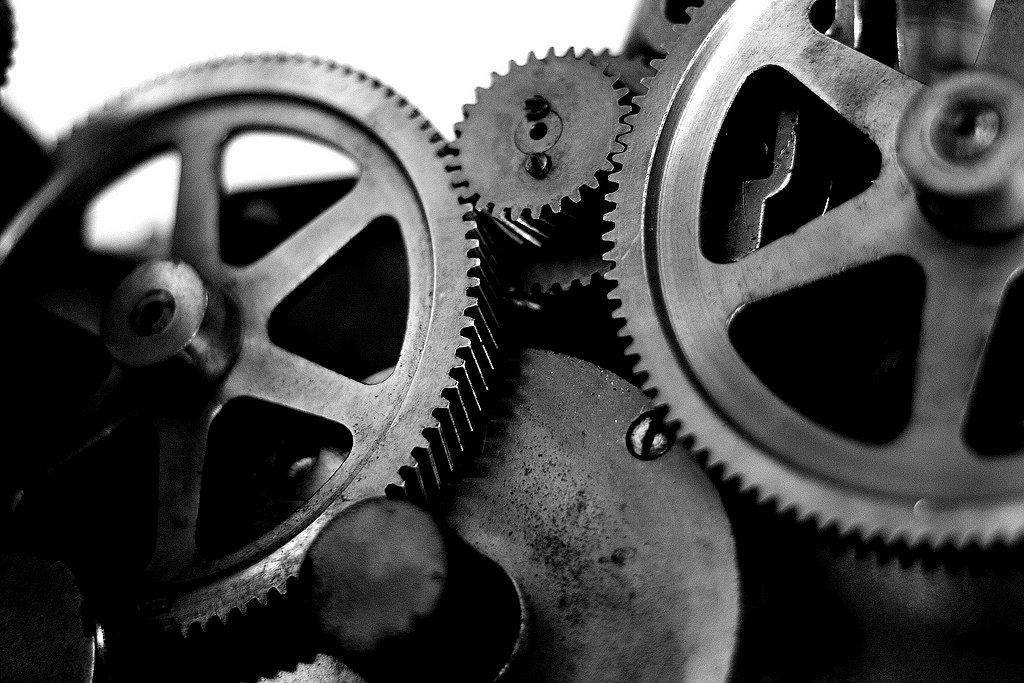
\includegraphics[scale=.07]{images/spur_gear.png}& & \\ \hline 
			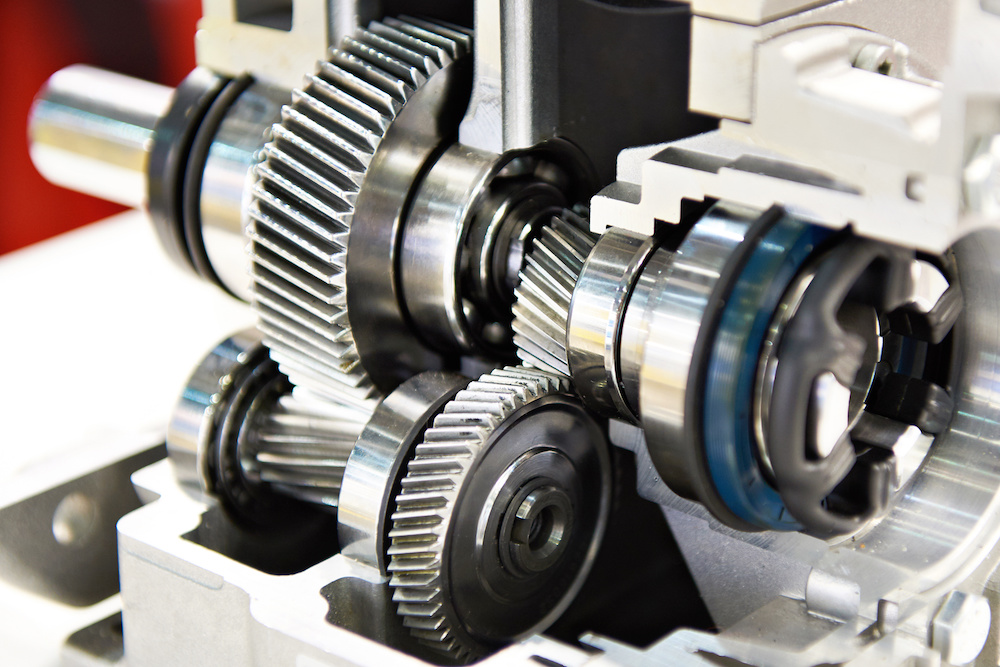
\includegraphics[scale=.35]{images/helical_gear.png}& & \\ \hline
			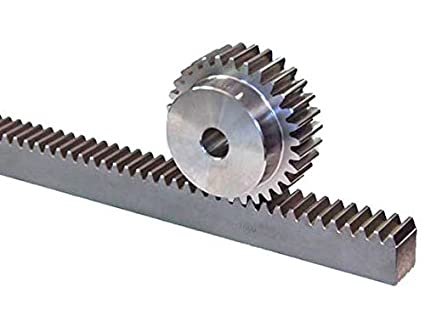
\includegraphics[scale=.65]{images/rack_and_pinion2.png}& & \\ \hline
			& & \\
			



		\end{tabular}

		{\tiny images:\href{https://commons.wikimedia.org/w/index.php?search=gear&title=Special:MediaSearch&go=Go&type=image}{wikimedia commons} }

	\end{frame}

	% Section I - Frame III
	\begin{frame} \small
		\frametitle{\sectiontitleI}

		Alternatives:
		\begin{itemize}
				\item 
				\item
				\item
        \end{itemize}


        \begin{multicols}{2}
		\underline{Pros}
		\begin{itemize}
		\item
		\item
		\item
		\end{itemize}
		\underline{Cons}
		\begin{itemize}
		\item 
		\item
		\item
		\end{itemize}
		\end{multicols}

	\end{frame}

	
% Section II
\section{\sectiontitleII}	

	% Section II - Frame I
	\begin{frame}[label=sectionI] \small
		\frametitle{\sectiontitleII}

		   	\begin{itemize}
					\item 
					\item
					\item
	        \end{itemize}

		\end{frame}

	% Section II - Frame II
	\begin{frame} \small
		\frametitle{\sectiontitleII}
		
		   	\begin{itemize}
					\item 
					\item
					\item
	        \end{itemize}
            
  	\end{frame}
		

% Section III
\section{\sectiontitleIII}	

	% Section III - Frame I
	\begin{frame}[label=sectionIII] \small
		\frametitle{\sectiontitleIII}
	 
	       \begin{itemize}
	            \item 
	            \item 
	            \item 
	            \item 
	        \end{itemize}

		\end{frame}  
	
% Section IV	
\section{\sectiontitleIV}	
	% Section IV - Frame I
	    \begin{frame}[label=sectionIV] \small
		\frametitle{\sectiontitleIV}    
  
  			\begin{itemize}
	            \item 
	            \item 
	            \item 
	            \item 
	        \end{itemize}

		\end{frame}
		
\end{document}